\newlecture[Fixed Income Securities][Sep 21, 2026]

\begin{definition}[Financial Instruments]
    A legal obligation or claim having monetary value (eg. mortage, stocks and bonds...)
\end{definition}
\begin{definition}[Security]
    A tradable financial instrument satisfying legal and regulatory requirements.
\end{definition}
\begin{definition}[Fixed Income Securities]
    Securities that promise a fixed income to the holder over some spam of time. (eg. bonds, mortages, annuities)
\end{definition}

\heading{Annuity}
A contract that pays the holder money periodically according to the fixed schedule.
\\\b{Perpetual Annuity (Perpetuity)} - Pays a fixed sum periodically, forever.

\begin{center}
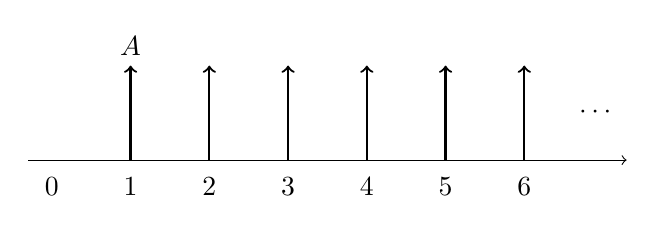
\begin{tikzpicture}
    \draw[->] (-0.3,0) -- (7.3,0);
    \foreach \x in {0,1,2,3,4,5,6} {
        \node[below] at (\x,-0.1) {\x};
    }
    \foreach \x in {1,2,3,4,5,6} {
        \draw[->, thick] (\x,0) -- (\x,1.2);
    }
    \node[above] at (1,1.2) {$A$};
    \node at (6.9,0.6) {$\cdots$};
\end{tikzpicture}
\end{center}

At a per period interest rate of $r$, the PV is
\[P = \sum_{k=1}^{\infty}\frac{A}{(1+r)^k} = \frac{A}{r}\]
Note: Infinite sum!!


\heading{Finite-Life Streams}
A stream that pays $A$ for $n$ periods, starting at period 1. What is the PV?

\begin{center}
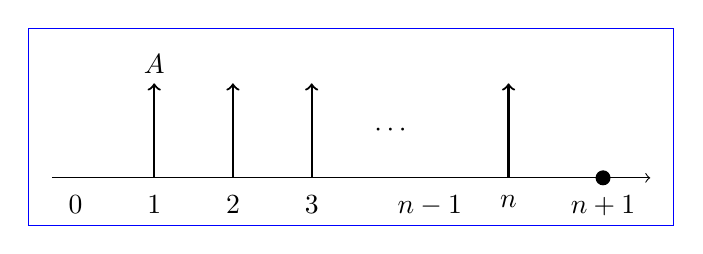
\begin{tikzpicture}
    \draw[blue] (-0.6,-0.6) rectangle (7.6,1.9);
    \draw[->] (-0.3,0) -- (7.3,0);
    \node[below] at (0,-0.1) {$0$};
    \node[below] at (1,-0.1) {$1$};
    \node[below] at (2,-0.1) {$2$};
    \node[below] at (3,-0.1) {$3$};
    \node[below] at (4.5,-0.1) {$n-1$};
    \node[below] at (5.5,-0.1) {$n$};
    \node[below] at (6.7,-0.1) {$n+1$};
    \draw[->, thick] (1,0) -- (1,1.2);
    \draw[->, thick] (2,0) -- (2,1.2);
    \draw[->, thick] (3,0) -- (3,1.2);
    \node at (4,0.6) {$\cdots$};
    \draw[->, thick] (5.5,0) -- (5.5,1.2);
    \filldraw (6.7,0) circle (2.5pt);
    \node[above] at (1,1.2) {$A$};
\end{tikzpicture}
\end{center}

\[\boxed{P = \sum_{k=1}^{n}\frac{A}{(1+r)^k} = \frac{A}{r}\left(1-\frac{1}{(1+r)^n}\right)}\]
where $r$ is the interest rate per period.

A finite life-stream can be thought as the \underline{difference between two perpetuities}.

Perpetuity starting at period 1:
\begin{center}
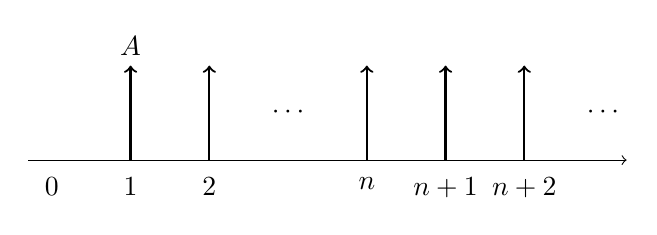
\begin{tikzpicture}
    \draw[->] (-0.3,0) -- (7.3,0);
    \node[below] at (0,-0.1) {$0$};
    \node[below] at (1,-0.1) {$1$};
    \node[below] at (2,-0.1) {$2$};
    \node[below] at (4,-0.1) {$n$};
    \node[below] at (5,-0.1) {$n+1$};
    \node[below] at (6,-0.1) {$n+2$};
    \draw[->, thick] (1,0) -- (1,1.2);
    \draw[->, thick] (2,0) -- (2,1.2);
    \draw[->, thick] (4,0) -- (4,1.2);
    \draw[->, thick] (5,0) -- (5,1.2);
    \draw[->, thick] (6,0) -- (6,1.2);
    \node at (3,0.6) {$\cdots$};
    \node at (7,0.6) {$\cdots$};
    \node[above] at (1,1.2) {$A$};
\end{tikzpicture}
\end{center}

Perpetuity starting at period $n+1$:
\begin{center}
\begin{tikzpicture}
    \draw[->] (-0.3,0) -- (7.3,0);
    \node[below] at (0,-0.1) {$0$};
    \node[below] at (1,-0.1) {$1$};
    \node[below] at (2,-0.1) {$2$};
    \node[below] at (4,-0.1) {$n$};
    \node[below] at (5,-0.1) {$n+1$};
    \node[below] at (6,-0.1) {$n+2$};
    \draw[->, thick] (5,0) -- (5,1.2);
    \draw[->, thick] (6,0) -- (6,1.2);
    \node at (3,0.6) {$\cdots$};
    \node at (7,0.6) {$\cdots$};
    \node[above] at (5,1.2) {$A$};
\end{tikzpicture}
\end{center}
\[PV = \frac{A}{r} - \frac{A}{r}\left(\frac{1}{(1+r)^n}\right)\]
\[PV_{fin} = \frac{A}{r}\left(1 - \frac{1}{(1+r)^n}\right)\]


\begin{example}[Loan Calculation]
    Suppose \$1,000 is borrowed at 12\% interest compounded monthly, repayed with equal monthly payments over 5 years. How much are the monthly payments?

    Given: $P = \$1,000 \quad r = \frac{12\%}{12} = 1\%/\text{mo} \quad n = 5\times12 = 60$
    \[P = \frac{A}{r}\left(1-\frac{1}{(1+r)^n}\right) \quad \Rightarrow \quad A = \frac{rP}{\left(1-\frac{1}{(1+r)^n}\right)} = \$22.24/\text{mo}\]
\end{example}

\header{Bonds}
An agreement to pay money according to the rules of the issue.
\\Generally, bonds have\begin{itemize}
    \item Face Value, Par Value, Principal - an amount to be paid at the maturity date.
    \item Coupon Payments - an amount paid periodically, expressed as a \% of the face value. Last coupon is paid at maturity.
\end{itemize}

\begin{example}
    Given:
    \[\text{Face Value } = \$1,000 \qquad \text{Coupon } = 9\%\]
    The yearly coupon amount is $\$1,000(0.09) = \$90$
\end{example}

\header{Payoff Structure of a Bond}
\begin{center}
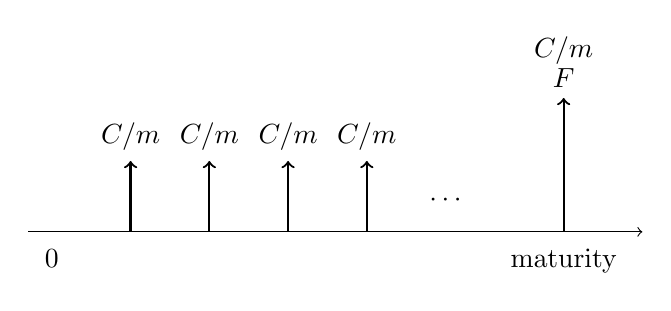
\begin{tikzpicture}
    \draw[->] (-0.3,0) -- (7.5,0);
    \node[below] at (0,-0.1) {$0$};
    \node[below] at (6.5,-0.1) {maturity};
    \draw[->, thick] (1,0) -- (1,0.9) node[above] {$C/m$};
    \draw[->, thick] (2,0) -- (2,0.9) node[above] {$C/m$};
    \draw[->, thick] (3,0) -- (3,0.9) node[above] {$C/m$};
    \draw[->, thick] (4,0) -- (4,0.9) node[above] {$C/m$};
    \node at (5,0.4) {$\cdots$};
    \draw[->, thick] (6.5,0) -- (6.5,1.7);
    \node at (6.5,2.3) {$C/m$};
    \node at (6.5,1.95) {$F$};
\end{tikzpicture}
\end{center}

where $C$ is the annual coupon amount, and $F$ is the face value.

When there are no coupons, the only payoff is the face value at maturity.

\begin{center}
\begin{tikzpicture}
    \draw[->] (-0.3,0) -- (7.5,0);
    \node[below] at (0,-0.1) {$0$};
    \node[below] at (6.5,-0.1) {maturity};
    \node at (3.5,0.4) {$\cdots$};
    \draw[->, thick] (6.5,0) -- (6.5,1.2) node[above] {$F$};
\end{tikzpicture}
\end{center}

This is known as a \b{zero-coupon bond}, or a zero.

\header{Accrued Interest}
Ignored by bond price quotes, but must be added to the price.

\begin{center}
\begin{tikzpicture}
    \draw[->] (-0.3,0) -- (8.5,0);
    \draw[->, thick] (0,0) -- (0,1.3) node[above] {$C/m$};
    \draw[->, thick] (8,0) -- (8,1.3) node[above] {$C/m$};
    \draw[decorate, decoration={brace, amplitude=6pt}] (0.3,0.85) -- (7.7,0.85) node[midway, above=8pt] {$t_c$};
    \draw[decorate, decoration={brace, mirror, amplitude=6pt}] (0,-0.3) -- (5,-0.3) node[midway, below=8pt] {$t$};
    \draw[->] (6.2,-1.6) -- (5.1,-0.2);
    \node[below] at (6.6,-1.7) {you purchase};
\end{tikzpicture}
\end{center}

You must pay the previous owner their ``portion'' of the next coupon payment.

\[\boxed{AI = \frac{\text{days since last coupon}}{\text{days in current coupon period}} \times (C/m) = \frac{t}{t_c}(C/m)}\]